\documentclass[a4paper, 12pt]{report}
\usepackage{cmap}
\usepackage[T2A]{fontenc}
\usepackage[utf8]{inputenc}
\usepackage[english,russian]{babel}
\usepackage{listings}
\usepackage{amsmath}
\usepackage{float}
\usepackage{csquotes}
\usepackage{graphicx}
\graphicspath{ {./images/} }
\usepackage{xcolor}
\definecolor{buzzlightyear}{HTML}{8757A5}
\definecolor{grass}{HTML}{738D06}
\definecolor{literal}{HTML}{F18A2B}
\definecolor{commentcolor}{HTML}{8E908B}

\lstdefinestyle{habrstyle}{
	backgroundcolor=\color{white},
	commentstyle=\color{commentcolor},
	keywordstyle=\bfseries\color{buzzlightyear},
	numberstyle=\tiny\color{commentcolor},
	stringstyle=\color{grass},
	basicstyle=\ttfamily\footnotesize,
	breakatwhitespace=false,         
    	breaklines=true,                 
   	captionpos=b,                    
    	keepspaces=true,                 
    	numbers=left,                    
    	numbersep=7pt,                  
    	showspaces=false,                
    	showstringspaces=false,
   	showtabs=false,                  
    	tabsize=3
}

\lstset{style=habrstyle}

\author{3530901/80201, Шелаев Н. Р.}
\title{Лабораторная работа № 8. Фильтрация и свертка.}
\date{\today}

\begin{document}
	\maketitle
	\tableofcontents
	\listoffigures
	\lstlistoflistings

	\chapter{Сглаживание}
	Это операция, удаляющая быстрые изменения сигнала для выявления общих зависимостей.
	Попробуем это на чём-нибудь применить.
	\begin{lstlisting}[language=Python,caption=Воспользуемся акциями Facebook]
		import pandas as pd

		df = pd.read_csv('FB_2.csv', header=0, parse_dates=[0])
		close = df['Close']
		dates = df['Date']
		days = (dates - dates[0]) / np.timedelta64(1,'D')
		M = 30
		window = np.ones(M)
		window /= sum(window)
		smoothed = np.convolve(close, window, mode='valid')
		smoothed_days = days[M // 2:(len(smoothed) + M // 2)]
		plt.plot(days, close, color = 'gray', alpha = 0.6, label = 'daily close')
		plt.plot(smoothed_days, smoothed, color = 'C1', alpha = 0.6, label = '30 day average')
	\end{lstlisting}
	\begin{figure}[H]
		\centering
		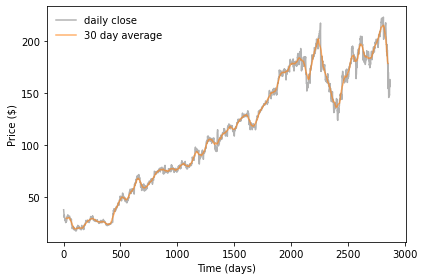
\includegraphics[width=0.75\textwidth]{test1.png}
		\caption{Результат работы сглаживания}
		\label{fig:test1}
	\end{figure}
	\begin{lstlisting}[language=Python,caption=А теперь реальный сигнал]
		from thinkdsp import SawtoothSignal

		signal = SawtoothSignal(freq = 440)
		wave = signal.make_wave(duration=1.0, framerate=44100)
		window = np.ones(11)
		window /= sum(window)
		plt.plot(window)
		segment = wave.segment(duration = 0.01)
		segment.plot()
	\end{lstlisting}
	\begin{figure}[H]
		\centering
		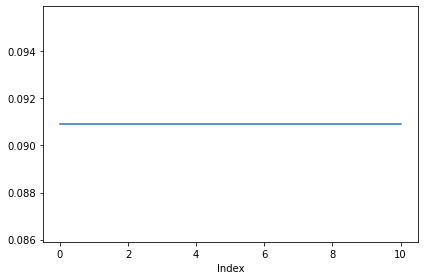
\includegraphics[width=0.75\textwidth]{test2.png}
		\caption{Окно сигнала}
		\label{fig:test2}
	\end{figure}
	\begin{figure}[H]
		\centering
		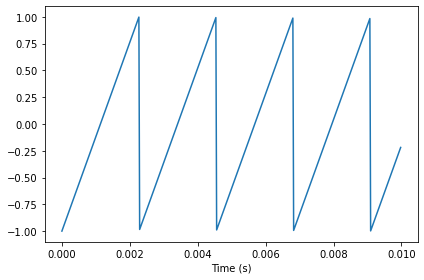
\includegraphics[width=0.75\textwidth]{test3.png}
		\caption{Сегмент пилообразного сигнала}
		\label{fig:test3}
	\end{figure}
	\begin{lstlisting}[language=Python,caption=Сделали нужную ширину окна]
		def zero_pad(array, n):
			res = np.zeros(n)
			res[:len(array)] = array
			return res

		N = len(segment)
		padded = zero_pad(window, N)
		plt.plot(padded)
	\end{lstlisting}
	\begin{figure}[H]
		\centering
		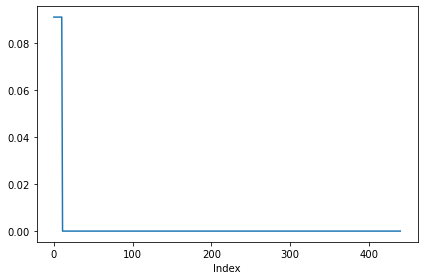
\includegraphics[width=0.75\textwidth]{test4.png}
		\caption{Изменили ширину окна}
		\label{fig:test4}
	\end{figure}
	\begin{lstlisting}[language=Python,caption=Сдвинули окно вправо]
		prod = padded * segment.ys
		smoothed = np.zeros(N)
		rolled = padded.copy()
		for i in range(N):
			smoothed[i] = sum(rolled * segment.ys)
			rolled = np.roll(rolled, 1)
		
		plt.plot(rolled)
	\end{lstlisting}
	\begin{figure}[H]
		\centering
		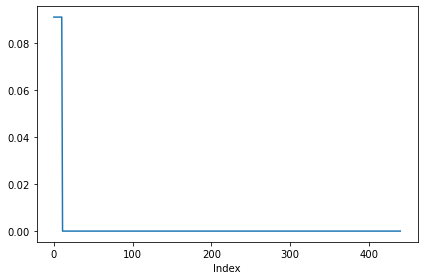
\includegraphics[width=0.75\textwidth]{test5.png}
		\caption{Сдвиг окна}
		\label{fig:test5}
	\end{figure}
	\begin{lstlisting}[language=Python,caption=Сравнение с исходным сигналом]
		from thinkdsp import Wave

		segment.plot(color = 'gray')
		smooth = Wave(smoothed, framerate = wave.framerate)
		smooth.plot()
	\end{lstlisting}
	\begin{figure}[H]
		\centering
		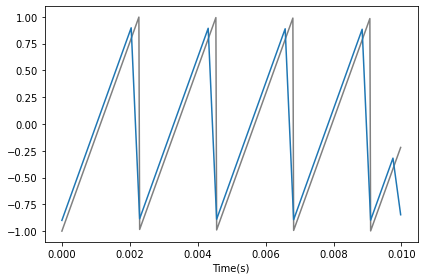
\includegraphics[width=0.75\textwidth]{test6.png}
		\caption{В правой части что-то не так}
		\label{fig:test6}
	\end{figure}
	\begin{lstlisting}[language=Python,caption=Встроенная функция свертки]
		segment.plot(color = 'gray')
		ys = np.convolve(segment.ys, window, mode = 'valid')
		smooth2 = Wave(ys, framerate = wave.framerate)
		smooth2.plot()
	\end{lstlisting}
	\begin{figure}[H]
		\centering
		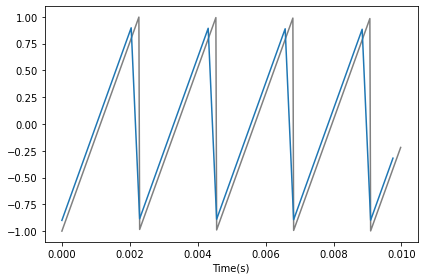
\includegraphics[width=0.75\textwidth]{test7.png}
		\caption{Так-то лучше}
		\label{fig:test7}
	\end{figure}

	\chapter{Частотная область}
	Как операция сглаживания влияет на спектр сигнала?
	\begin{lstlisting}[language=Python,caption=Сравнение исходного и сглаженного сигнала]
		convolved = np.convolve(wave.ys, window, mode = 'same')
		smooth = Wave(convolved, framerate = wave.framerate)
		spectrum = wave.make_spectrum()
		spectrum.plot(color = 'gray')
		spectrum2 = smooth.make_spectrum()
		spectrum2.plot()
	\end{lstlisting}
	\begin{figure}[H]
		\centering
		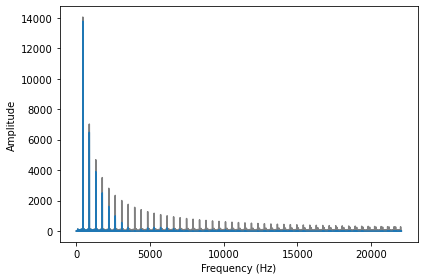
\includegraphics[width=0.75\textwidth]{test8.png}
		\caption{Результат сглаживания}
		\label{fig:test8}
	\end{figure}
	\begin{lstlisting}[language=Python,caption=Соотношение спектров сигнала до и после сглаживания]
		amps = spectrum.amps
		amps2 = spectrum2.amps
		ratio = amps2 / amps    
		ratio[amps < 280] = 0
		padded = zero_pad(window, len(wave))
		dft_window = np.fft.rfft(padded)
		plt.plot(np.abs(dft_window), color = 'gray', label = 'DFT(window)')
		plt.plot(ratio, label = 'amplitude ratio')
	\end{lstlisting}
	\begin{figure}[H]
		\centering
		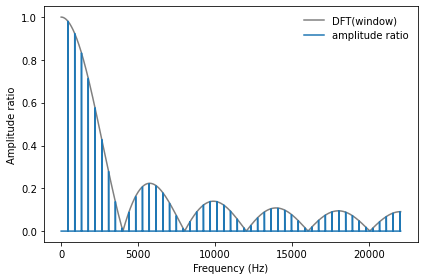
\includegraphics[width=0.75\textwidth]{test9.png}
		\caption{График соотношения спектров до и после сглаживания}
		\label{fig:test9}
	\end{figure}

	\chapter{Гауссов фильтр}
	Протестируем работу гауссова филльтра на различных сигналах.
	\begin{lstlisting}[language=Python,caption=Прямоугольное и гауссово окна]
		import scipy.signal		

		boxcar = np.ones(11)
		boxcar /= sum(boxcar)
		gaussian = scipy.signal.gaussian(M = 11, std = 2)
		gaussian /= sum(gaussian)
		plt.plot(boxcar, label = 'boxcar')
		plt.plot(gaussian, label = 'Gaussian')
	\end{lstlisting}
	\begin{figure}[H]
		\centering
		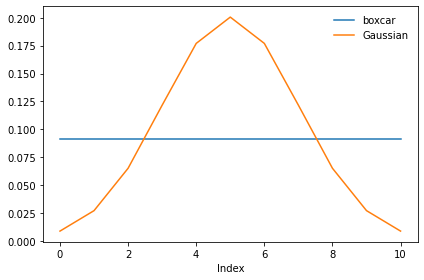
\includegraphics[width=0.75\textwidth]{test10.png}
		\caption{Результат сравнения двух окон}
		\label{fig:test10}
	\end{figure}
	\begin{lstlisting}[language=Python,caption=Собрали всё в одну функцию]
		from thinkdsp import SquareSignal

		def plot_filter(M = 11, std = 2):
			signal = SquareSignal(freq = 440)
			wave = signal.make_wave(duration=1, framerate=44100)
			spectrum = wave.make_spectrum()
			gaussian = scipy.signal.gaussian(M = M, std = std)
			gaussian /= sum(gaussian)
			ys = np.convolve(wave.ys, gaussian, mode = 'same')
			smooth = Wave(ys, framerate = wave.framerate)
			spectrum2 = smooth.make_spectrum()
			amps = spectrum.amps
			amps2 = spectrum2.amps
			ratio = amps2 / amps    
			ratio[amps < 560] = 0
			padded =  zero_pad(gaussian, len(wave))
			dft_gaussian = np.fft.rfft(padded)		
			plt.plot(np.abs(dft_gaussian), color = 'gray', label = 'Gaussian filter')
			plt.plot(ratio, label = 'amplitude ratio')

		slider = widgets.IntSlider(min=2, max=100, value=11)
		slider2 = widgets.FloatSlider(min=0, max=20, value=2)
		interact(plot_filter, M = slider, std = slider2);
	\end{lstlisting}
	\begin{figure}[H]
		\centering
		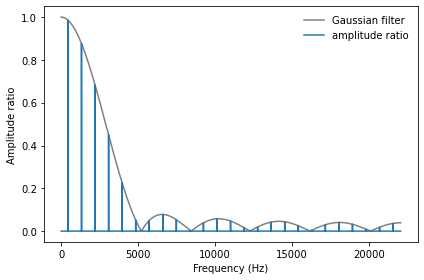
\includegraphics[width=0.75\textwidth]{test11.png}
		\caption{Исследование зависимости результата от значений M и std}
		\label{fig:test11}
	\end{figure}
	При увеличении \texttt{std} без увеличения \texttt{M} можно заметить, что \textquote{скачки} снова появляются, как если бы мы взяли \texttt{Boxcar}-фильтр на \texttt{M} элементов.

	\chapter{Эффективная свертка}
	Улучшаем алгоритм свертки.
	\begin{lstlisting}[language=Python,caption=Исходная свертка]
		window = scipy.signal.gaussian(M = 30, std = 6)
		window /= window.sum()
		smoothed = np.convolve(close, window, mode = 'valid')
		plt.plot(close, color = 'gray')
		plt.plot(smoothed)
	\end{lstlisting}
	\begin{figure}[H]
		\centering
		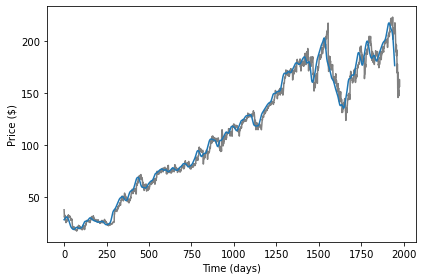
\includegraphics[width=0.75\textwidth]{test12.png}
		\caption{Надо улучшить!}
		\label{fig:test12}
	\end{figure}
	\begin{lstlisting}[language=Python,caption=Улучшаем алгоритм свертки]
		N = len(close)
		padded = zero_pad(window, N)
		fft_window = np.fft.fft(padded)
		plt.plot(np.abs(fft_window))
		fft_signal = np.fft.fft(close)
		smoothed2 = np.fft.ifft(fft_signal * fft_window)
		M = len(window)
		smoothed2 = smoothed2[M-1:]
		plt.plot(smoothed)
		plt.plot(smoothed2.real)
	\end{lstlisting}
	\begin{figure}[H]
		\centering
		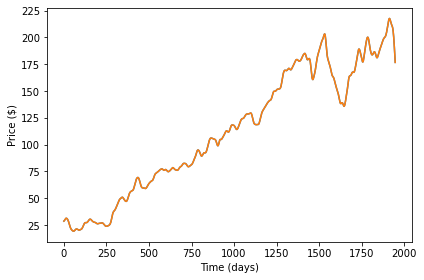
\includegraphics[width=0.75\textwidth]{test13.png}
		\caption{Почти полное совпадение!}
		\label{fig:test13}
	\end{figure}
	Сравнили этот алгоритм с встроенным алгоритмом \sloppy{\texttt{np.fft.fft}}. Разница между результатами близка к 0.
	
	\chapter{Эффективная автокорреляция}
	А теперь улучшим алгоритм автокорреляции.
	\begin{lstlisting}[language=Python,caption=Улучшенная автокорреляция]
		corrs = np.correlate(close, close, mode = 'same')

		def fft_autocorr(signal):
			N = len(signal)
			signal = zero_pad(signal, 2 * N)
			window = np.flipud(signal)
			corrs = fft_convolve(signal, window)
			corrs = np.roll(corrs, (N // 2 + 1))[:N]
			return corrs

		corrs2 = fft_autocorr(close)
		lags = np.arange(N) - N // 2
		plt.plot(lags, corrs, color = 'gray', alpha = 0.5, label = 'np.convolve')
		plt.plot(lags, corrs2.real, color = 'C1', alpha = 0.5, label = 'fft_convolve')
	\end{lstlisting}
	\begin{figure}[H]
		\centering
		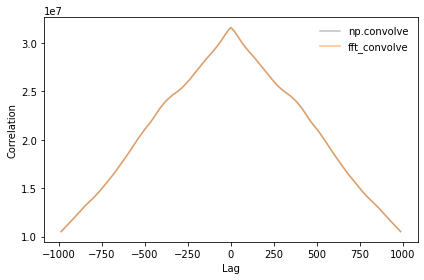
\includegraphics[width=0.75\textwidth]{test14.png}
		\caption{Сравнение двух алгоритмов}
		\label{fig:test14}
	\end{figure}
	Разница между этими двумя алгоритмами близка к 0.
	
	\chapter{Упражнения}
	\section{Задание 2}
	Исследование преобразования Фурье над сигналами нормального распределения.
	\begin{lstlisting}[language=Python,caption=Получение сигнала]
		import scipy.signal

		gaussian = scipy.signal.gaussian(M = 32, std = 2)
		gaussian /= sum(gaussian)
		plt.plot(gaussian)
		fft_gaussian = np.fft.fft(gaussian)
		plt.plot(abs(fft_gaussian))
	\end{lstlisting}
	\begin{figure}[H]
		\centering
		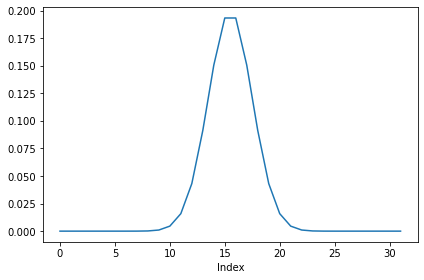
\includegraphics[width=0.75\textwidth]{task1.png}
		\caption{Исходный сигнал}
		\label{fig:task1}
	\end{figure}
	\begin{figure}[H]
		\centering
		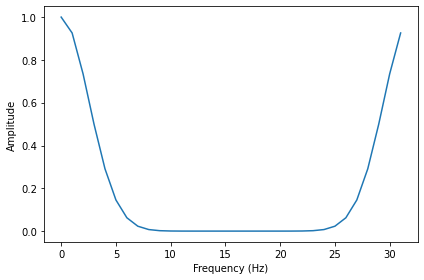
\includegraphics[width=0.75\textwidth]{task2.png}
		\caption{Применение функции FFT}
		\label{fig:task2}
	\end{figure}
	\begin{lstlisting}[language=Python,caption=Сдвинули отрицательные частоты влево]
		N = len(gaussian)
		fft_rolled = np.roll(fft_gaussian, N // 2)
		plt.plot(abs(fft_rolled))
	\end{lstlisting}
	\begin{figure}[H]
		\centering
		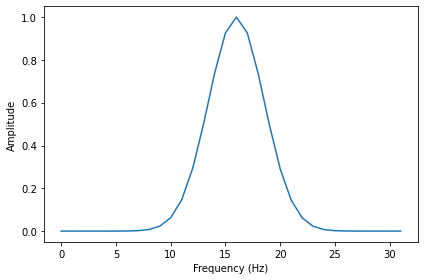
\includegraphics[width=0.75\textwidth]{task3.png}
		\caption{Немного измененный сигнал}
		\label{fig:task3}
	\end{figure}
	\begin{lstlisting}[language=Python,caption=Исследование влияния значения std]
		def plot_gaussian(std):
			M = 32
			gaussian = scipy.signal.gaussian(M = M, std = std)
			gaussian /= sum(gaussian)
			plt.subplot(1, 2, 1)
			plt.plot(gaussian)
			decorate(xlabel = 'Time')
			fft_gaussian = np.fft.fft(gaussian)
			fft_rolled = np.roll(fft_gaussian, M // 2)
			plt.subplot(1, 2, 2)
			plt.plot(np.abs(fft_rolled))

		slider = widgets.FloatSlider(min=0.1, max=10, value=2)
		interact(plot_gaussian, std = slider);
	\end{lstlisting}
	\begin{figure}[H]
		\centering
		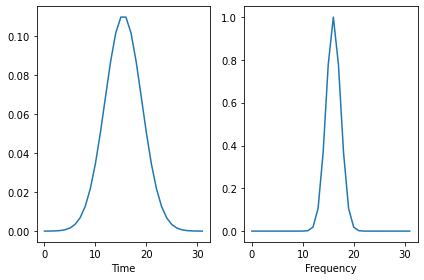
\includegraphics[width=1.0\textwidth]{task4.png}
		\caption{Изменяем значение std}
		\label{fig:task4}
	\end{figure}
	При увеличении значения \sloppy{\texttt{std}} левый \textquote{колокол} расширяется, а правый - сужается, и наоборот.

	\section{Задание 3}
	Более подробно исследуем различные окна.
	\begin{lstlisting}[language=Python,caption=Начало исследования]
		from thinkdsp import SquareSignal

		signal = SquareSignal(freq = 440)
		wave = signal.make_wave(duration=1.0, framerate=44100)
		M = 25
		std = 5.0
		gaussian = scipy.signal.gaussian(M = M, std = std)   
		bartlett = np.bartlett(M)
		blackman = np.blackman(M)
		hamming = np.hamming(M)
		hanning = np.hanning(M)
		windows = [blackman, gaussian, hanning, hamming]
		names = ['blackman', 'gaussian', 'hanning', 'hamming']

		for window in windows: window /= sum(window)

		for window, name in zip(windows, names):
			plt.plot(window, label=name)
	\end{lstlisting}
	\begin{figure}[H]
		\centering
		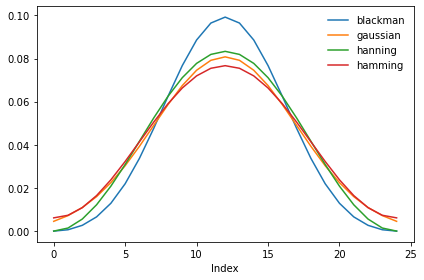
\includegraphics[width=0.75\textwidth]{task5.png}
		\caption{Применение окон к исходному сигналу}
		\label{fig:task5}
	\end{figure}
	\begin{lstlisting}[language=Python,caption=Применение функции DFT]
		def zero_pad(array, n):
			res = np.zeros(n)
			res[:len(array)] = array
			return res

		def plot_window_dfts(windows, names):
			for window, name in zip(windows, names):
				padded = zero_pad(window, len(wave))
				dft_window = np.fft.rfft(padded)
				plt.plot(abs(dft_window), label = name)

		plot_window_dfts(windows, names)
	\end{lstlisting}
	\begin{figure}[H]
		\centering
		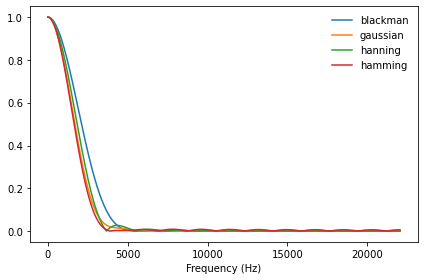
\includegraphics[width=0.75\textwidth]{task6.png}
		\caption{Результаты сравнения}
		\label{fig:task6}
	\end{figure}
	Все функции очень похожи, однако, можно отметить, что функция Хэмминга падает быстрее всех, а Блэкмана - медленнее всех.
	\begin{lstlisting}[language=Python,caption=Логарифмический масштаб]
		plot_window_dfts(windows, names)
		decorate(xlabel = 'Frequency (Hz)', yscale = 'log')
	\end{lstlisting}
	\begin{figure}[H]
		\centering
		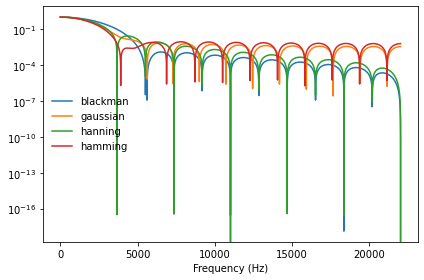
\includegraphics[width=0.75\textwidth]{task7.png}
		\caption{Результаты сравнения в логарифмическом масштабе}
		\label{fig:task7}
	\end{figure}
	В этом масштабе мы заметили, что функции Хэмминга и Хамминга падают быстрее всех. Окна Хэмминга и Гаусса имеют самые стойкие боковые лепестки. 

	\chapter{Вывод}
	В данной работе мы рассмотрели схлаживание сигналов, улучшили алгоритмы свертки и автокорреляции. В последнем упражнении  сравнили работу 4-х различных окон.
\end{document}